
\subsubsection{24.10.14}

\begin{enumerate}
	\item Время начала и окончания собрания:
	16:00 - 20:00
	\item Цели собрания:
	\begin{enumerate}
	  \item Устарнить баг сервопривода.
	  
	  \item Изготовить из приобретенного нами листа алюминия и установить откосы для мячей в виде балок, расположенных в форме воронки в передней части робота.
	  
    \end{enumerate}
    
	\item Проделанная работа:
	\begin{enumerate}
	  \item Баг сервопривода устарнен. Причина его возникновения - вращение сервопривода после остановки с небольшой скоростью, которой не хватало на преодоление силы упругости стяжек. Связано это с нерпавильным значением мощности сервопривода в коде (значение, в котором сервопривод не вращается - 127 вместо стоявшего у нас 135).
      
      \item Лист алюминия распилен на полосы нужной длины и ширины.
      
      \item Откосы установлены на робота и протестированы. Результат положительный.
      
      \item При тестировании откосов было замечено, что при столкновении с жестким препятствием они изгибаются. Для предотвращения этого были установлены упоры выпиленные из алюминиевой полосы.
      
      \begin{figure}[H]
      	\begin{minipage}[h]{0.47\linewidth}
      		\center{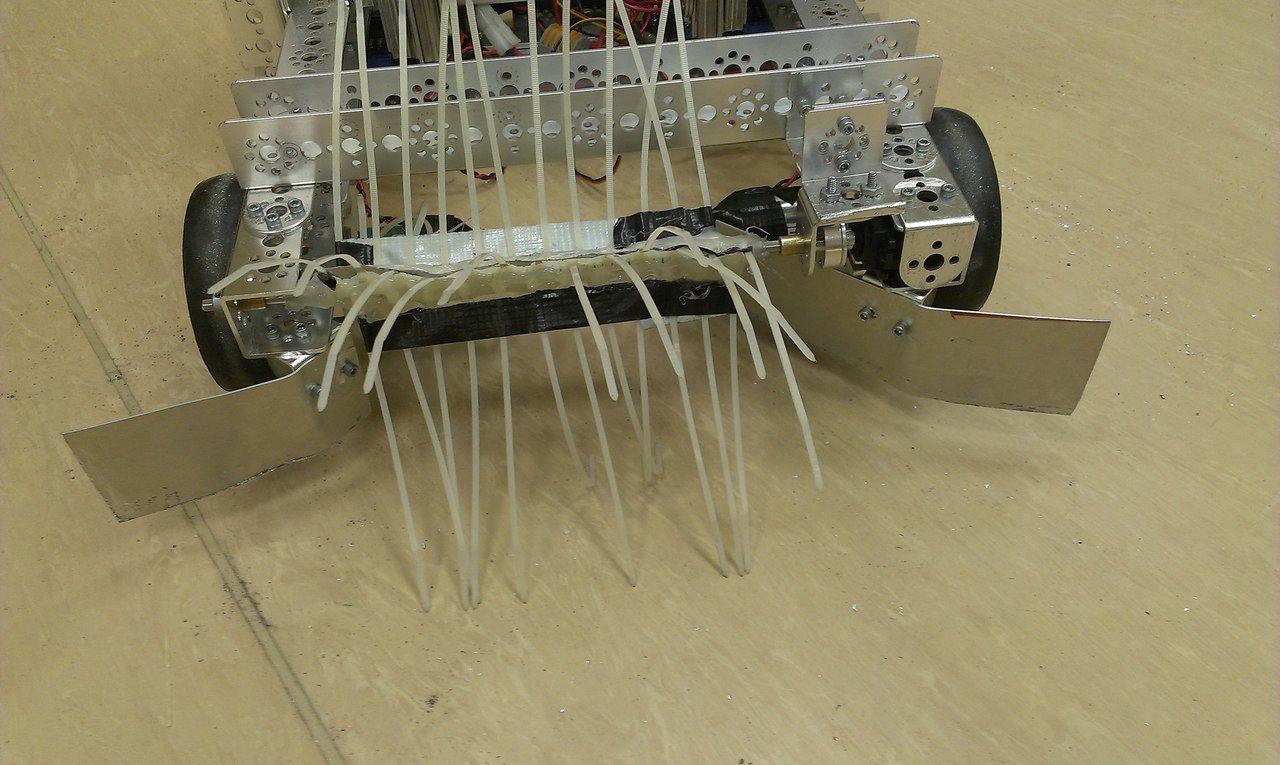
\includegraphics[scale=0.2]{days/images/7E29mPyMEKE}}
      		\caption{Захват с откосами}
      	\end{minipage}
      	\hfill
      	\begin{minipage}[h]{0.47\linewidth}
      		\center{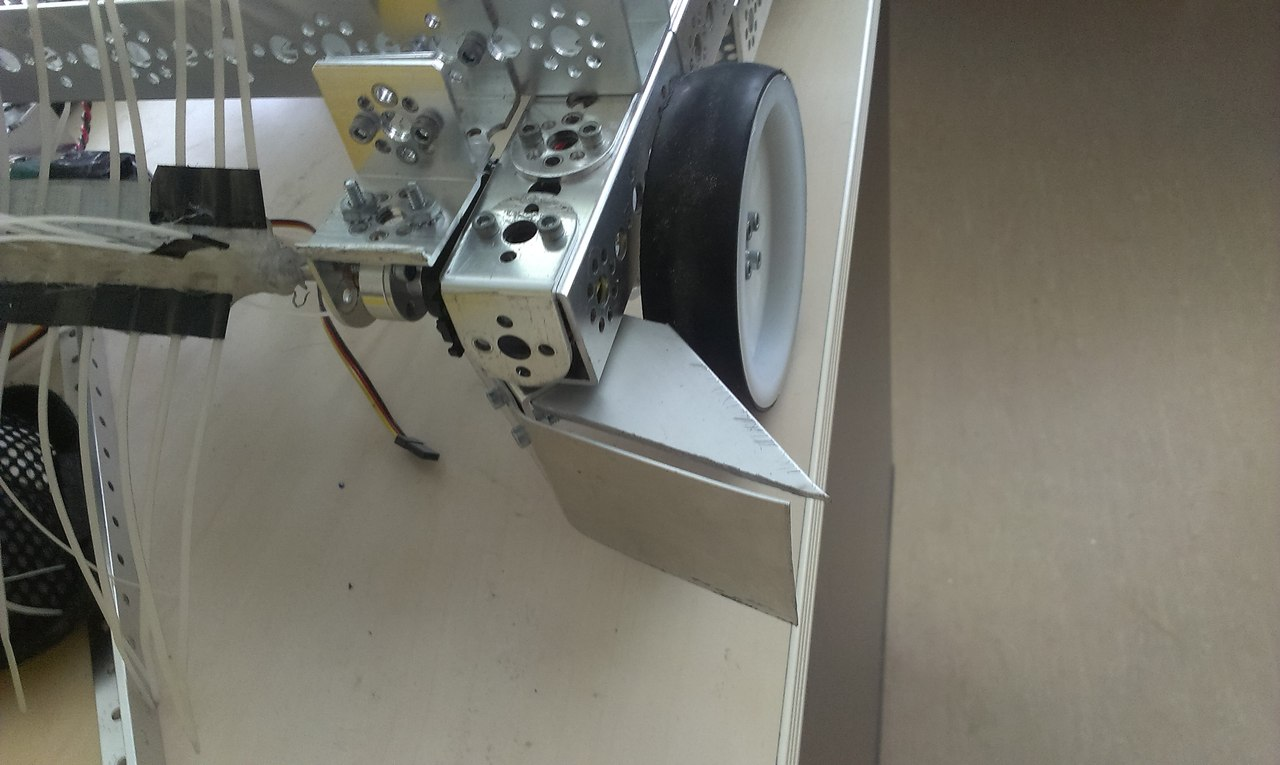
\includegraphics[scale=0.2]{days/images/_82S9xrm9y4}}
      		\caption{Откосы укреплены упорами}
      	\end{minipage}
      \end{figure}
      
      \item Подготовлены отверстия для установки оставшейся пары поперечных перекладин на подъемнике.
      
    \end{enumerate}
    
	\item Итоги собрания: 
	\begin{enumerate}
	  \item Баг сервопривода устранен.
	  
      \item Откосы для мячей установлены на робота.
      
    \end{enumerate}
    
	\item Задачи для последующих собраний:
	\begin{enumerate}
	  \item Спроектировать и создать механизм захвата передвижных корзин.
	  
    \end{enumerate}     
\end{enumerate}

\fillpage
